

\documentclass[aspectratio=169, 12pt]{beamer}

%%%%%%%%%%%%
% Packages %
%%%%%%%%%%%%

\usepackage{ctex}
\usepackage[english]{babel}
\usepackage{packages/sleek}
\usepackage{packages/tweaks}
\usepackage{calligra} % thanks pakeage

%%%%%%%%%%%%%%%%
% Bibliography %
%%%%%%%%%%%%%%%%

\addbibresource{./resources/bib/references.bib}

%%%%%%%%%%%%%%
% Title-page %
%%%%%%%%%%%%%%


\title{公共经济学}
\subtitle{Based on Metropolis theme}
\author[LIU ShHUAI]{刘 {  } 帅}
\institute{山西师范大学 {  } 经济与管理学院}
\date{\today}
\titlelogo{./resources/pdf/logo.png}
\framelogo{./resources/pdf/logo.png}

%%%%%%%%%%%%
% Document %
%%%%%%%%%%%%

\begin{document}

\maketitle

\begin{frame}[standout]
    案例分析二\par
    \addtolength{\parskip}{.4em}
    邻避冲突的外部性理论解释及其治理策略
\end{frame}

\begin{frame}[plain]
    % \begin{multicols}{1}
    %   \frametitle{Outline}
    %   \tableofcontents[hideallsubsections]
    % \end{multicols}
    \frametitle{Outline}
    \tableofcontents[hideallsubsections]
    % \tableofcontents[currentsection]
  \end{frame}

\section{内容提要}

\begin{frame}[plain]
    \frametitle{内容提要}
    邻避冲突是影响社会稳定的风险因素之一。本章以昆明市民反对PX项目事
件为例,界定了邻避效应、邻避设施、邻避冲突、邻避型群体性事件等概念,以外
部性理论为基础,提出“邻避设施外部性导致邻避冲突出现——邻避设施不对
称博弈导致邻避冲突升级——公众权利意识增强导致邻避冲突群体化”的演变
过程;在借鉴国外邻避冲突治理经验的基础上,构建我国邻避冲突治理的行为
理念、体制框架和运行机制。
\end{frame}

\section{一、引言}

\begin{frame}{plain}
    \frametitle{导入案例}
    2013年5月,发生在昆明市的两次市民聚集游行事件,受到国内外媒体的
广泛关注。2013年5月4日,约3000名市民在昆明市中心的南屏街聚集游行,
抗议中国石油天然气集团公司(简称中国石油)云南1000万吨炼油项目在昆明
安宁市落户;游行群众对这一石油炼化项目特别是其下游产品对二甲苯项目
(简称PX项目)表现出抵制情绪,在现场高举“还我美丽昆明!我们要生存!
我们要健康”等标语,表达对PX项目的不满,要求政府相关部门加强项目信
息公开和环保监督。
\end{frame}

\begin{frame}{plain}
    \frametitle{导入案例}
    因这一诉求未得到完全满足,2013年5月16日,千余名群
众于市中心老省政府所在的五华山再次聚集游行,游行队伍以“散步”的形式,
途径正义坊、金碧路,到达西昌路。昆明市市长李文荣在西昌路上与游行队伍对
话,并承诺于17日中午12时前开通新浪微博与网友对话,并于5月21日重新
与市民座谈。
\end{frame}

\begin{frame}[plain]
    \frametitle{导入案例}
    根据昆明市环境保护局公布的《中国石油云南1000万吨/年炼油项目环境影
响评价第二次公示》,中国石油云南1000万吨/年炼油项目位于昆明市下辖的安宁市草铺镇境内。项目总投资193.34亿元,其中建设投资156.08 亿元,环保投
资13.30亿元,工程建设期为2-4年,预期2014年2月建成投产。
\end{frame}

\begin{frame}[plain]
    \frametitle{导入案例}
    昆明市民反对PX 项目事件是典型的邻避冲突事件。1980 年,英国记者
Emilie在描述美国人对居住区周围堆积的化工垃圾警觉与反感现象时,首次提
出了“邻避”一词;在之后的研究中,把给公众带来正效益的同时也给设施
周边居民制造负效益的设施称为邻避设施。邻避设施的收益由全体社会成员共
同享受,而其负外部性成本则由生活在设施周边的居民承担,且对设施周边居
民而言,邻避设施建设带来的成本往往大于收益;但对于整个社会而言邻避设
施建设带来的总收益大于总成本(含负外部性成本),是资源配置的帕累托改
进,因此,邻避设施周边居民通过正常的意见反馈渠道,往往难以促使政府或
其他组织更改邻避设施的选址。为了维护自身的基本权益,邻避设施周边居民尝试通过集体行动方式来表达其诉求,从而形成一种“邻避冲突”。
\end{frame}

\begin{frame}[plain]
    \frametitle{导入案例}
    国内外学者的研究中提供了丰富的邻避冲突治理策略,但是与中国现实国
情相结合、具有可操作性的邻避冲突治理对策仍显不足,以至于面对邻避冲突政
府往往只是采取两种简单策略:
\par
一是“停”,如2012年10月22日宁波镇
海发生反对PX项目的群体性事件,宁波市政府最终做出“坚决不上PX项目;
炼化一体化项目前期工作停止推进,再作科学论证”的决策;2013年7月12日
广东江门鹤山市约千名民众上街反对在该市兴建核燃料项目,次日鹤山市政府
决定对该项目不予申请立项。
\end{frame}

\begin{frame}[plain]
    \frametitle{导入案例}
    二是“迁”,如厦门市沧海PX项目最终迁址漳州;
北京西二旗垃圾场建设项目在附近居民的联名反对声中决定选址重建,原项目
建设地将改为城市绿地。邻避设施“停”建损害了整个社会的收益;邻避设施
“迁”建损害了新址周边居民的收益。“停”和“迁”都没有解决邻避设施带来
的社会冲突或减少社会收益损失,且昆明市民反对PX项目事件在可提前“预
知”的前提下出现,因此,仍需基于现有研究成果,在分析邻避冲突产生原因
的基础上,进一步探索邻避冲突的治理策略。
\end{frame}

\section{二、概念界定}

\begin{frame}{plain}
    \frametitle{邻避效应(Not In My Backyard)}
    当国家推行垃圾场、核电站、殡仪馆、化工厂等对社会整体而言具有必要性的项目时,由于项目建设地居民因担心项目建设对环境、健康、固定资产等带来负面影响,从而滋生“不要建在我家后院”的心理,进而强烈反对把当地作为项目实施地,甚至采取强烈集体性抗争行为的草根运动,这一现象称为邻避效应。
    \par
    邻避效应反映了特定范围内的居民自我矛盾的态度:他们原则上赞成政府建设对社会整体而言有必要性的垃圾场、核电站、殡仪馆、化工厂等项目,但是不同意把这些项目建设在自己周边。
\end{frame}

\begin{frame}{plain}
    \frametitle{邻避设施}
    邻避设施特质能够在给公众带来正效益的同时也给周边居民制造负效应的设施,如核电站、精神病院、监狱、石油化工厂、垃圾场等都属于邻避设施。邻避设施有两个显著特征:
    \par
    一是同时产生正外部性与负外部性;
    \par
    二是成本和收益的不对称性。从整体角度计算,邻避设施的正外部性大于负外部性,但对于生活在邻避设施周围的居民而言,负外部性大于正外部性。
\end{frame}

\begin{frame}[plain]
    \frametitle{邻避冲突}
    由于公众对邻避设施建设的不满程度加剧而产生的在邻避设施周边居民、政府、邻避设施建设单位之间的冲突成为邻避冲突,它具有高度感性特征。生活在邻避设施周围的居民,很容易产生受到社会体系排挤的想法,一旦有呼吁者就能调动他们的反抗情绪,而且这种反抗情绪不受科学知识的约束,即使政府或专家发布项目可行的论证信息,邻避冲突往往也不会因之而平息。
\end{frame}

\begin{frame}[plain]
    \frametitle{邻避型群体性事件}
    由于邻避冲突扩大而引起的群体性事件称为邻避型群体性事件。生活在邻避设施周边的居民因担心邻避设施带来的负外部性而采取反抗的行动,形成邻避冲突;因单一的或小规模的邻避冲突不能解决邻避问题,开始动员更多的居民参与邻避冲突,甚至通过互联网手段动员没有生活在邻避设施周围的居民也参与邻避冲突,采取集体一致的行动策略,最终形成邻避型群众性事件。
\end{frame}

\section{三、邻避冲突的成因及其演化过程}

\begin{frame}[plain]
    \frametitle{(一)邻避设施的外部性导致邻避冲突出现}
    外部性是指经济活动中私人边际成本与社会边际成本的不一致,即某些个人或厂商的经济行为影响了其他个人或厂商,却没有为之承担应有的成本费用或没有获得相应报酬的现象。按照外部性的效果,可以分为正外性与负外部性。正外部性是指在经济活动中私人边际成本于社会边际成本或者私人边际收益小于社会边际收益的情况。负外部性是指私人边际成本小于社会边际成本或者私人边际收益大于社会边际收益的现象,即个人或厂商的经济行为影响了其他个人或者厂商,却没有为之付出必要的成本。
\end{frame}

\begin{frame}[plain]
    \frametitle{(一)邻避设施的外部性导致邻避冲突出现}
    对于整个社会而言,邻避设施往往具有正的外部性。以昆明PX项目为例,建设昆明PX项目,能够填补云南省的产业空白,带动数千亿的GDP增量,且有利于建成云南省石油、磷、盐、氯碱化工共同发展的大产业循环圈,降低成本、减少污染。借助边际外部收益的概念,设昆明PX项目的产量为Q,价格为P,边际社会成本为MSC,边际私人成本为MPC,边际私人收益为MPR,边际外部收益为MER,供给曲线为S,需求曲线为D,如下图所示:
\end{frame}

\begin{frame}[plain]
    \frametitle{(一)邻避设施的外部性导致邻避冲突出现}
    \begin{figure}
        \centering
        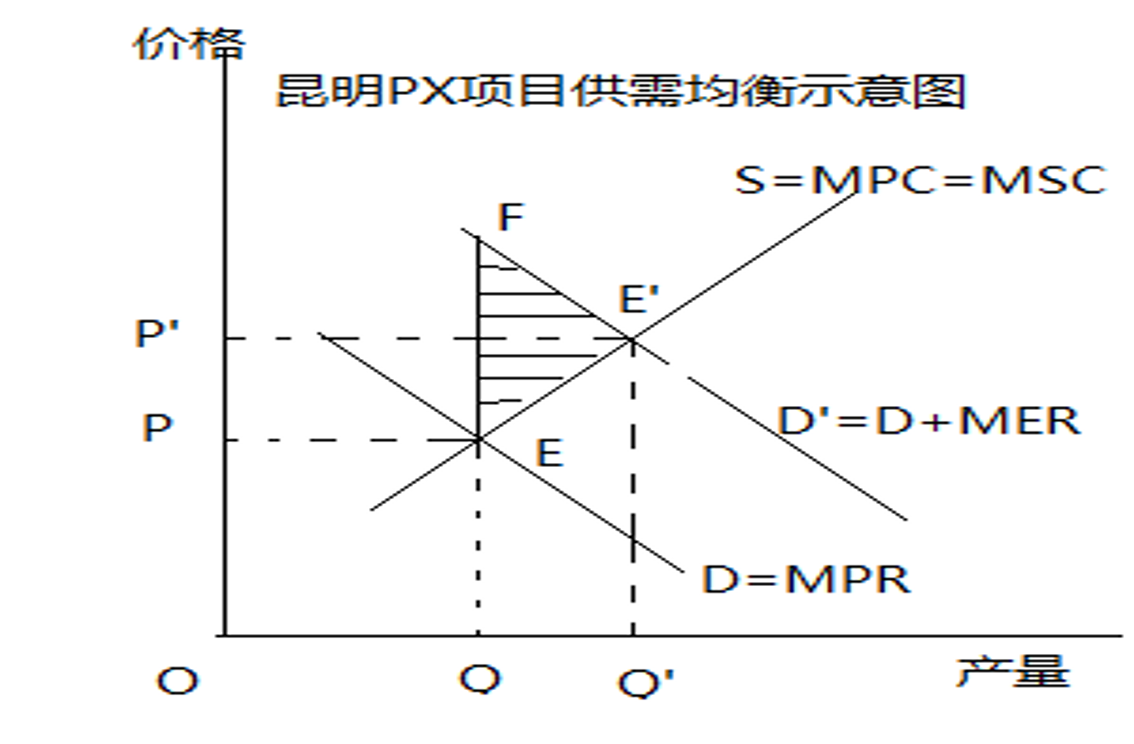
\includegraphics[width=0.8\textwidth]{./resources/figure/notinmybackyard.png}
        \end{figure}
\end{frame}

\begin{frame}[plain]
    \frametitle{(一)邻避设施的外部性导致邻避冲突出现}
    假设昆明px项目的边际私人成本和边际社会成本相等,在上图中,S是以边际私人成本为基础的供给曲线,D是以边际私人收益为基础的需求曲线,两者的交点为E,形成此时的均衡价格为P和均衡产量Q。但是E点并没有处于帕累托最优状态,如果考虑边际外部收益MER,PX项目的生产均衡点为E’,价格为P’,产量为Q’。
\end{frame}

\begin{frame}[plain]
    \frametitle{(一)邻避设施的外部性导致邻避冲突出现}
    此时价格P低于P’,产量Q也小于Q’。说明由于存在正外部性,厂商世纪提供的产量小于帕累托最优状态的产量。对待邻避设施供给,往往需要由政府出面引导建设。正是由于这一原因,造就了邻避冲突产生的一个要件,即政府主导邻避设施建设。
    \par
    当邻避设施周边居民反对邻避设施建设、政府不会轻易放弃自己主导的邻避设施建设两个条件同时成立时,因为邻避设施的外部性而产生的邻避冲突具有不可避免性。
\end{frame}

\begin{frame}[plain]
    \frametitle{(二)邻避设施建设的不对称博弈导致邻避冲突升级}
    邻避设施建设涉及的利益主体包括政府、邻避设施周边居民、邻避设施施工方、论证专家。由于政府在邻避设施建设中的主导作用,可以代表邻避设施施工方、论证专家与邻避设施周边居民博弈,即博弈双方是政府和邻避设施周边居民。政府具有公共政策制定权,掌握着丰富的资源,在博弈中处于强势地位。
\end{frame}

\begin{frame}[plain]
    \frametitle{(二)邻避设施建设的不对称博弈导致邻避冲突升级}
    居民很少能够参与到邻避设施的建设决策过程中,对邻避设施的规划、危害、收益等信息知之甚少,社会参与能力和信息掌握程度都不能与政府相比,在博弈中处于劣势地位。按照常规的博弈方式与程序,邻避设施周边居民往往达不成利益诉求的目的。在博弈过程中,政府的软肋在于上级政府的强制性“维稳”要求,因而将邻避冲突扩大到超过上级政府强制性“维稳”的上限,就成为邻避设施周边居民不得不采取的博弈策略,即邻避设施建设的不对称博弈导致邻避冲突的升级。
\end{frame}

\begin{frame}[plain]
    \frametitle{(三)公众权利意识增强导致邻避冲突群体化}
    非邻避设施周边居民参与、信息传递方式多样化、提前告知群体性活动方案等特征反映了共众权利意识的增强。邻避设施周边居民因邻避设施带来的危害而主动维权;非邻避设施周边居民出于社会公平正义理念而参与维权;采取多种措施传递信息,说明公众维权能力的提高;提前告知群体性活动方案反映了居民对维护合法权益而采取集体活动的正当性认知。这些反映公众权利意识增强的因素,最终导致邻避冲突向邻避型群体性事件转化。
\end{frame}

\section{四、国外治理邻避冲突的经验}

\begin{frame}[plain]
    \frametitle{(一)促进邻避冲突双方的有效沟通}
    瑞典成立了核能安全机关与辐射保护局,该局设立专门科室负责与民众沟通,体现政府的信息透明已取得公众信任。瑞典政府设计的风险沟通模式,包括风险评估、民间组织参与、公众参与、信息发布等模块,已经被多个欧盟国家借鉴已解决邻避设施争议。
\end{frame}

\begin{frame}[plain]
    \frametitle{(一)促进邻避冲突双方的有效沟通}
    公众对邻避设施抗争的原因之一是不了解邻避设施的真是危害性,对邻避设施所带来的风险不确定性有自我夸大意识。这就要求政府作为博弈双方中的信息强势者,把邻避设施相关信息充分的与公众沟通,告知公众邻避设施的真是收益与风险。
\end{frame}

\begin{frame}[plain]
    \frametitle{(二)加强公众参与邻避设施决策的力度}
    在邻避设施选址建设前,德国采取“共识会议”制度,政府代表、公众代表、施工方代表、专家学者齐聚一堂,相互沟通、对话、讨论,公众的意见和建议对邻避设施选址和建设发挥着重要作用。公众能够参与到邻避设施规划、补偿、建设等各个环节,虽然付出了较高的时间成本,但是为邻避冲突的解决提供了范本。
    \par
    我国邻避设施建设应当借鉴国外和台湾地区的经验,建立从选址到建设整个决策链条的公众参与机制,不能等到邻避冲突爆发才让公众参与进来,以预防、减少社会冲突,促进社会稳定。
\end{frame}

\begin{frame}[plain]
    \frametitle{(三)完善防止利益冲突的制度建设}
    第一,重视价值观导向,规定公职人员必须树立正确的民主价值、职业价值、伦理价值和做人价值观念;
    \par
    第二,注重制度约束,建立起资产申报、资产处理、离职后行为限制、利益回避、设立利益冲突处理专员等制度;
    \par
    第三,着力加强教育培训。
    \par
    我国在避邻冲突治理过程中,应当借鉴加拿大的经验,制定关于邻避冲突治理的法律法规,防止邻避效应上升为邻避型群体性事件。
\end{frame}

\section{五、邻避冲突的治理策略}

\begin{frame}[plain]
    \frametitle{(一)邻避冲突治理的行为理念}
    新公共管理运动时20世纪80年代兴起于英、美等国的一种新的公共管理模式,基本内容是:
    \par
    第一,以顾客为导向,奉行顾客至上的价值理念。
    \par
    第二,转变政府职能,把管理和具体操作分开,政府只是制定政策而不是执行政策。
    \par
    第三,在公共管理中引入竞争机制,让更多的私营部门参与提供公共服务。
    \par
    第四,借鉴私营部门的成功经验,重视公共服务提供效率,实施绩效管理。第五,改革公务员制度,推行合同制和临时雇佣制度。第六,创造有事业心和有预见性的政府,政府要学会以花钱来省钱、以回报定投资,在作出重要决定时,要有预见性。
\end{frame}

\begin{frame}[plain]
    \frametitle{(二)邻避冲突治理的体制框架}
    邻避冲突的演化过程可以分为邻避设施政府立项的潜伏期、邻避设施选址的诞生期、邻避冲突升级的成长期、邻避型群体性事件出现的转化期、邻避冲突平息后的善后期。邻避冲突演化的五个阶段需要不同的政府部门参与,建立多元协作的邻避冲突治理体制框架。
\end{frame}

\begin{frame}[plain]
    \frametitle{(三)邻避冲突治理的运行机制}
    (1)邻避设施负外部性的补偿机制
    \par
    以外部效应内部化为基础,对邻避设施可能出现的负外部性进行全面的评估,对已经发生的损失和将要发生的损失进行补偿,以最大限度的降低居民对邻避设施的反对情绪。利用税费政策对污染严重的企业征收一定的环境税费;明晰当地居民拥有不受污染的河流、土地、空气的生存权利,采用货币补偿和非货币补偿相结合的办法,给予邻避设施周边居民以经济利益、工作机会、医疗服务等方面的补偿,形成行之有效的邻避设施负外部性界定、评估、测算、补偿程序。
\end{frame}

\begin{frame}[plain]
    \frametitle{(三)邻避冲突治理的运行机制}
    (2)邻避设施建设的信息公开机制
    \par
      对于类似项目的建设,政府应当公开项目的选址、安全性、对环境的影响等信息,并保证决策程序的透明,接受当地居民和非政府公共组织的监管,防止利益集团和寻租行为影响公共决策。
    \par
      (3)邻避设施建设的公众参与机制
    \par
      邻避设施建设不仅是技术层面的问题,而且使社会层面的问题。要充分了解公众对邻避设施风险的评估、风险承受意愿、风险与收益的权衡态度等。邻避设施建设决策应当去政治化,建立起邻避设施周边居民参与邻避设施决策的正常机制。
\end{frame}

\begin{frame}[plain]
    \frametitle{(三)邻避冲突治理的运行机制}
    (4)邻避设施建设的风险理性培育机制
    邻避冲突的出现具有感性特征。参与邻避冲突的居民往往自行夸大邻避设施的风险,并散播风险言论,引发更大范围的邻避冲突。应当借助风险沟通、评估平台,建立起具有集体意识、科学合理的公众风险认知和对待风险的态度。加强社会风险宣传与教育,引导公众树立正确的风险观。    
\end{frame}

% ---------------------------------------------------------------------------
\begin{frame}[standout]
    \begin{center}
        {\Huge\calligra Thanks!}
      \end{center}
\end{frame}
% ---------------------------------------------------------------------------

\end{document}
